%! TEX root = Calculo.tex
\documentclass{../Calculo.tex}


\begin{document}
\section{Bibliografía}
\begin{itemize}
	\item Stewart, J. Cálculo en varias variables.
	\item Apuntes de Pepe Aranda.
	\item Tom M. Apostol, "Calculus".
	\item Tom M. Apostol, Análisis Matemático.
\end{itemize}
\pagebreak
\chapter{El espacio Rn}
\section{El conjunto $\R^{n}$}
$\R^{n}$ es el conjunto
\[
		\R^{n} =\{ ( x_1,\dots ,x_{n}) / x_{i} \in \R, 1 \leq i \leq n\}
\]
De momento, este conjunto no tiene ninguna estructura. Para ello, se introduce
la noción de espacio vectorial (EV a partir de ahora).
\begin{itemize}
	\item La suma vectorial:
	\[
		\vec{a} + \vec{b} = (a_{i}+b_{i},\dots a_{n}+b_{n})	
	\]
	\item Producto por escalar:
		\[
			k \vec{a} = (ka_{1},\dots ,ka_{n})
		\]
\end{itemize}
Con estas dos operaciones, $\mathbb{R}^{n}$ es EV, y a sus elementos, los vamos a
llamar vectores, y los denotaremos por $\vec{x}=(x_{1},\dots x_{n})$.\\
Con esta estructura, los elementos de $\mathbb{R}^{n}$ se pueden ordenar, por
ejemplo, en una cuadrícula.
\begin{center}

\tikzset{every picture/.style={line width=0.75pt}} %set default line width to 0.75pt        

\begin{tikzpicture}[x=0.75pt,y=0.75pt,yscale=-1,xscale=1]
%uncomment if require: \path (0,300); %set diagram left start at 0, and has height of 300

%Straight Lines [id:da3051942297151431] 
\draw    (231,181) -- (345,181) ;
\draw [shift={(347,181)}, rotate = 180] [color={rgb, 255:red, 0; green, 0; blue, 0 }  ][line width=0.75]    (10.93,-3.29) .. controls (6.95,-1.4) and (3.31,-0.3) .. (0,0) .. controls (3.31,0.3) and (6.95,1.4) .. (10.93,3.29)   ;
%Straight Lines [id:da9246749315532883] 
\draw    (231,181) -- (307.83,74.62) ;
\draw [shift={(309,73)}, rotate = 125.84] [color={rgb, 255:red, 0; green, 0; blue, 0 }  ][line width=0.75]    (10.93,-3.29) .. controls (6.95,-1.4) and (3.31,-0.3) .. (0,0) .. controls (3.31,0.3) and (6.95,1.4) .. (10.93,3.29)   ;




\end{tikzpicture}	
\end{center}

\subsection{$\mathbb{R}^{n}$ como espacio afín}
Nos será útil para definir direcciones desde cualquier punto de $\mathbb{R}^{n}$.
La estructura afín en $\mathbb{R}^{n}$ se define por la aplicación
\[
	\varphi: \mathbb{R}^{n} \times \mathbb{R}^{n} \mapsto \mathbb{R}^{n}
\]
\[
	(\vec{u}, \vec{v}) \mapsto \varphi(\vec{u}, \vec{v})
\]
donde $\varphi(\vec{u}, \vec{v})$ se representará como un vector cuyo punto
de aplicación está en el extremo de $\vec{u}$ y el extremo, el de $\varphi(
\vec{u}, \vec{v})$ en el extremo de $\vec{v}$. Es fácil comprobar que
\[
	\varphi(\vec{u},\vec{v}) = \vec{v} - \vec{u}
\]
En este contexto es conveniente llamar puntos a los vectores con punto de
aplicación en el $\vec{0}$ y vectores a los vectores cuyo punto de aplicación
es arbitratio. Los puntos también los denotaremos mediante letras mayúsculas,
y los vectores con letras minúsculas.
\begin{center}
	

\tikzset{every picture/.style={line width=0.75pt}} %set default line width to 0.75pt        

\begin{tikzpicture}[x=0.75pt,y=0.75pt,yscale=-1,xscale=1]
%uncomment if require: \path (0,300); %set diagram left start at 0, and has height of 300

%Straight Lines [id:da9620131632250988] 
\draw    (251,201) -- (367,201) ;
%Straight Lines [id:da5426532654970737] 
\draw    (251,201) -- (329,93) ;
%Straight Lines [id:da23784315263106715] 
\draw [color={rgb, 255:red, 0; green, 0; blue, 0 }  ,draw opacity=1 ]   (367,201) -- (329.66,94.89) ;
\draw [shift={(329,93)}, rotate = 70.62] [color={rgb, 255:red, 0; green, 0; blue, 0 }  ,draw opacity=1 ][line width=0.75]    (10.93,-3.29) .. controls (6.95,-1.4) and (3.31,-0.3) .. (0,0) .. controls (3.31,0.3) and (6.95,1.4) .. (10.93,3.29)   ;

% Text Node
\draw (387,203.4) node [anchor=north west][inner sep=0.75pt]    {$P$};
% Text Node
\draw (294,58.4) node [anchor=north west][inner sep=0.75pt]    {$Q$};
% Text Node
\draw (357,110.4) node [anchor=north west][inner sep=0.75pt]    {$\varphi ( P,Q) =\overrightarrow{PQ}$};


\end{tikzpicture}
\end{center}
A recordar que punto - punto define un vector, y que punto + vector = punto.
Con esto ya podemos definir direcciones.
\subsection{$\mathbb{R}^{n}$ como espacio métrico}
Para medir longitudes, ángulos y distancias introduciremos en $\mathbb{R}^{n}$
el \textbf{producto escalar}.
\begin{defin}
	El producto escalar entre dos vectores $\vec{u}$ y $\vec{v}$ se define como
	\[
		\cdot : \mathbb{R}^{n} \times  \mathbb{R}^{n} \mapsto \mathbb{R}
	\]
	\begin{equation}
		\begin{split}
			\vec{u} \cdot  \vec{v} = \sum_{i=1}^{n} u_{i}v_{i}
		\end{split}
	\end{equation}
	El producto escalar tiene las propiedades siguientes:
	\begin{itemize}
		\item $\vec{u} \cdot  \vec{v} = \vec{v} \cdot \vec{u}$
		\item $\vec{u} \cdot (\vec{v}+\lambda\vec{w})= 
			\vec{u} \cdot \vec{v} + \lambda \vec{u} \cdot \vec{w}$
		\item $\vec{u} \cdot \vec{u} \geq 0 \implies \vec{u} \cdot \vec{u}=0
			\iff \vec{u} = \vec{0}$ 
	\end{itemize}
\end{defin}
Debido a la propiedad 3, podemos definir la longitud (o norma) de un vector como
\begin{defin}
	La longitud o norma de un vector se define como:
	\begin{equation}
		\begin{split}
			|\vec{u}| = \sqrt{\vec{u} \cdot \vec{u}} = \sqrt{\sum_{i=1}^{n}
			u_{i}^{2}}
		\end{split}
	\end{equation}
	Las propiedades son que:
	\begin{itemize}
		\item $|\vec{v}| = 0 \iff \vec{v} = 0$
		\item $|\lambda \vec{u}| = |\lambda| |\vec{u}|$
		\item Desigualdad de Cauchy-Schwarz:
			\[
				|\vec{u} \cdot \vec{v}|\leq |\vec{u}||\vec{v}|
			\]
		\begin{proof}[Demostración]
			Observemos que si uno de los vectores es el vector nulo, entonces
			la desigualdad se satisface por igualdad, o también si ambos vectores
			son proporcionales entre sí. Supongamos entonces que $u$ y $v$ son LI.
			Eso significa que la ecuación $u=\lambda v$ no tiene solución.
			\[
				u - \lambda v = \vec{0}
			\]
			\[
				(u-\lambda v)(u-\lambda v) = 0
			\]
			\[
				u \cdot u - 2xu\cdot v+x^{2} v\cdot v=0
			\]
			Recordando la definición de norma queda
			\[
				x^{2}|v|^{2}-2xu\cdot v + |u|^{2}=0
			\]
			Ahora tenemos una ecuación de segundo grado en $x$. Como no puede
			tener solución, $b^{2}-4ac < 0$.
			\[
				(2u\cdot v)^{2} -4|v|^{2}|u|^{2} < 0
			\]
			\[
				2|u\cdot v| < 2|v||u|
			\]
			\[
				|u\cdot v|<|v||u|
			\]
			Como deben cumplirse ambas
			\begin{equation}
				\begin{split}
					|u\cdot v| \leq |v||u|
				\end{split}
			\end{equation}
		\end{proof}
		\item Desigualdad triangular
			\[
				|\vec{u}+\vec{v}| \leq |\vec{u}|+|\vec{v}|
			\]
		\begin{proof}[Demostración]
			Partimos de $u+v$
			\[
				(u+v)\cdot (u+v)=|u|^{2}+2u\cdot v+|v|^{2} = |u+v|^{2} \geq 0
			\]
			Por Cauchy-Schwarz, $u\cdot v\leq|u\cdot v| \leq |u|\cdot |v|$
			\[
				|u+v|^{2} \leq |u|^{2} + |v|^{2} + 2|u||v|
			\]
			\[
				|u+v|^{2} \leq (|u|+|v|)^{2}
			\]
			\[
				|u+v| \leq |u|+|v|
			\]
		\end{proof}
	\end{itemize}
\end{defin}
De especial importancia son los vectores con norma $1$, denominados como
\textbf{vectores unitarios}.
\begin{defin}
	Definimos como vectores unitarios a esos vectores $\vec{v}$ que cumplen que
	\begin{equation}
		\begin{split}
			|\vec{v}| = 1
		\end{split}
	\end{equation}
\end{defin}
Mediante la desigualdad de Cauchy-Schwarz, podemos obtener un método para medir
ángulos. Observemos que de C-S se deduce 
\begin{equation}
	\begin{split}
		||u||v|| \leq u\cdot v \leq |u||v|
	\end{split}
\end{equation}
Si ninguno de los vectores es el nulo, podemos dividir entre las normas
\begin{equation}
	\begin{split}
		-1\leq\frac{u\cdot v}{|u||v|} \leq 1
	\end{split}
\end{equation}
Entonces, como está acotada en $[-1,1]$, podemos definir el ángulo $\alpha$ entre
$u$ y $v$ como
\begin{defin}
	El ángulo $\alpha$ entre $u$ y $v$ como el ángulo que satisface
	\begin{equation}
		\begin{split}
			\cos \alpha = \frac{u\cdot v}{|u||v|}
		\end{split}
	\end{equation}
	donde $\alpha \in [0,\pi]$. Es de relevancia que $\alpha$ siempre se mide como
	el ángulo "interior" o el más pequeño.
	\begin{center}
		

\tikzset{every picture/.style={line width=0.75pt}} %set default line width to 0.75pt        

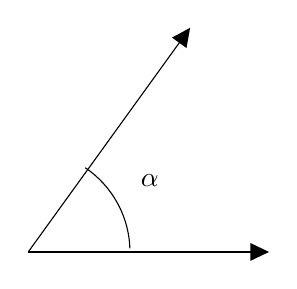
\begin{tikzpicture}[x=0.75pt,y=0.75pt,yscale=-1,xscale=1]
%uncomment if require: \path (0,300); %set diagram left start at 0, and has height of 300

%Straight Lines [id:da4204681338418119] 
\draw    (271,221) -- (384,221) ;
\draw [shift={(387,221)}, rotate = 180] [fill={rgb, 255:red, 0; green, 0; blue, 0 }  ][line width=0.08]  [draw opacity=0] (8.93,-4.29) -- (0,0) -- (8.93,4.29) -- cycle    ;
%Straight Lines [id:da9882209281394811] 
\draw    (271,221) -- (347.24,115.43) ;
\draw [shift={(349,113)}, rotate = 125.84] [fill={rgb, 255:red, 0; green, 0; blue, 0 }  ][line width=0.08]  [draw opacity=0] (8.93,-4.29) -- (0,0) -- (8.93,4.29) -- cycle    ;
%Shape: Arc [id:dp7205301342242372] 
\draw  [draw opacity=0] (298.46,180.41) .. controls (311.02,188.93) and (319.42,203.13) .. (319.97,219.32) -- (271,221) -- cycle ; \draw   (298.46,180.41) .. controls (311.02,188.93) and (319.42,203.13) .. (319.97,219.32) ;  

% Text Node
\draw (324,182.4) node [anchor=north west][inner sep=0.75pt]    {$\alpha $};


\end{tikzpicture}
	\end{center}
	Si $\alpha = \frac{\pi}{2} \implies u\cdot v = 0 \implies$ $u$ y $v$ son
	\textbf{ortogonales}.\\
	Aunque el ángulo entre $\vec{0}$ y otro vector cualquiera no está definido,
	sin embargo, se suele decir que $\vec{0}$ es ortogonal a todos los vectores de
	$\mathbb{R}^{n}$ 
\end{defin}
Ahora en $\mathbb{R}^{2}$ ya podemos dibujarlos "correctamente". Ahora falta
definir distancias entre puntos de $\mathbb{R}^{n}$.
\begin{defin}
	Definimos la distancia entre dos puntos $P$ y $Q$ como   
	\begin{equation}
		\begin{split}
			d(P,Q) = |\vv{PQ}| = |Q-P|
		\end{split}
	\end{equation}
\end{defin}
\subsection{Rectas e hiperplanos en $\mathbb{R}^{n}$}
Una recta en $\mathbb{R}^{n}$ que pasa por un punto $P$ y tiene la dirección
$\vv{v} \in \mathbb{R}^{n}$ se define como los puntos $X$ que satisfacen
\begin{equation}
	\begin{split}
		X = P+t\vv{v}
	\end{split}
\end{equation}
\begin{center}
	

\tikzset{every picture/.style={line width=0.75pt}} %set default line width to 0.75pt        

\begin{tikzpicture}[x=0.75pt,y=0.75pt,yscale=-1,xscale=1]
%uncomment if require: \path (0,300); %set diagram left start at 0, and has height of 300

%Straight Lines [id:da2796590956331695] 
\draw    (260,155) -- (401.11,106.65) ;
\draw [shift={(403,106)}, rotate = 161.09] [color={rgb, 255:red, 0; green, 0; blue, 0 }  ][line width=0.75]    (10.93,-3.29) .. controls (6.95,-1.4) and (3.31,-0.3) .. (0,0) .. controls (3.31,0.3) and (6.95,1.4) .. (10.93,3.29)   ;
%Straight Lines [id:da5188733313816549] 
\draw  [dash pattern={on 4.5pt off 4.5pt}]  (122,203) -- (514.53,68.5) ;

% Text Node
\draw (230,139.4) node [anchor=north west][inner sep=0.75pt]    {$P$};
% Text Node
\draw (337,66.4) node [anchor=north west][inner sep=0.75pt]    {$\vec{v}$};


\end{tikzpicture}
\end{center}
La recta está descrita por un solo parámetro libre, por lo que es un objeto de
dimensión $1$. Si $v_{j}\neq 0$ con $j \in \{ 1,\dots ,n \}$  podemos eliminar $t$
\begin{equation}
	\begin{split}
		t = \frac{x_{j}-p_{j}}{v_{j}}
	\end{split}
\end{equation}
Y entonces
\begin{equation}
	\begin{split}
		x_{i} = p_{i} +\frac{x_{j}-p_{j}}{v_{j}}v_{i} ~/~ i \neq j
	\end{split}
\end{equation}
Por tanto, la recta está definida por $n-1$ ecuaciones. Por tanto, la recta
es un objeto de codimensión $n-1$. 
\section{El símbolo de Levi-Civita o símbolo totalmente antisimétrico}
En $\mathbb{R}^n$ se define por:
$$
\varepsilon_{i, \dots, i_{n}}=  \left\{\begin{matrix}
1 &\text{ si } i_{i},\dots,i_{n}\text{ es una permutación par} \\
-1 &\text{si es una permutación impar}  \\
0 &\text{ en el resto de casos, cuando un índice se repite}  \\
\end{matrix}\right.
$$
$i_{1},\dots,i_{n}$ es una permutación par $123,\dots,n$ si para transformar una en otra necesitamos un número par de trasposiciones. Una trasposición es una permutación en la que solo se intercambian dos y solo dos elementos (no tienen por qué ser adyacentes).\\
Si queremos abusar todavía más de la notación, podemos usar el criterio de suma de Einstein. Este consiste en suponer que hay una suma siempre que un índice se repita, y la suma se hace en todo el rango de definición del índice:
$$
\mathbf{v} \cdot \mathbf{w} = v_{i} w_{i}
$$
\subsection{La delta de Kronecker}
$$
\delta_{ij}=  \left\{\begin{matrix}
1 & i=j \\
0 & i\neq j
\end{matrix}\right.
$$
Los vectores de la base canónica cumplen que:
$$
\mathbf{e}_{i}\cdot \mathbf{e}_{j}=\delta_{ij}
$$
Las bases cuyos vectores cumplan esto se dice que son bases \textbf{ortonormales}.
\section{Topología en $\mathbb{R}^{n}$}
\begin{defin}

Definimos un conjunto abierto de $\mathbb{R}^n$ a partir de la definición de bolas abiertas.\\
Dado $\mathbf{x}\in \mathbb{R}^n$ y dado $r\in \mathbb{R}^+$ se define la bola abierta centrada en $\mathbf{x}$ y de radio $r$ como el conjunto
$$
B_{r}(\mathbf{x})=\{ \mathbf{y}\in \mathbb{R}^n: d(\mathbf{x},\mathbf{y}) < r \}
$$
A veces convendrá usar bolas abiertas sin el punto central (perforadas), y se denotan por $B_{r}^*(\mathbf{x})$:
$$
B_{r}^*(\mathbf{x})=B_{r}(\mathbf{x})- \{ \mathbf{x} \}
$$
Un conjunto abierto $A\subset \mathbb{R}^n$ es abierto si y solo si para todo $\mathbf{x}\in A \exists \delta >0 : B_{\delta}(\mathbf{x})\subset A$
Además, se verifica que $ext(S)=\mathbb{R}^{n}-(S\cup\partial S)$
\end{defin}
\begin{defin}
Un conjunto $B\subset \mathbb{R}^n$ es cerrado si y solo si
$\mathbb{R}^n-B$ es abierto.
Además se verifica que $ext(B)=\mathbb{R}^{n}-B$
\end{defin}
Dado cualquier conjunto $S\subset \mathbb{R}^n$,podemos clasificar los puntos de $\mathbb{R}^n$ en:
\begin{itemize}
	\item Puntos interiores de $S$: si existe una bola centrada en dicho punto contenida en $S$.
	\item Puntos exteriores de $S$: si existe una bola centrada en el punto tal que $B(\mathbf{x},r) \cap S = \phi$.
	\item Puntos frontera de $S$: si $\forall r\in \mathbb{R}^{+} B(\mathbf{x},r)\cap S \neq \phi$ y $B(\mathbf{x},r)\cap(\mathbb{R}^n-S)\neq \phi$.
\end{itemize}
Todos estos conjuntos son disjuntos entre sí. Al conjunto de todos los puntos interiores de $S$ se les llama interior de $S$ y lo denotaremos por $int S$. Al conjunto de todos los puntos exteriores a $S$ se les llama exterior de $S$ y se denota por $ext S$. A los puntos frontera de $S$ se les llama frontera de $S$ y se denota por $\partial S$.
\begin{defin}
A $int(S)\cap\partial S$ se la denomina adherencia de $S$ y se denota por $\bar{S}$.
\end{defin}
\begin{defin}
A los puntos $\mathbf{x}$ que cumplen $B^{*}(\mathbf{x},r)\cap S\neq \phi$ se les llama puntos límite de $S$.
\end{defin}
\section{Funciones en $\mathbb{R}^{n}$ }
Sea
$$
f:D \subset \mathbb{R}^n\to \mathbb{R}^m
$$
Si $n=m=1$ entonces es una función de variable real. Si $n>1$ y $m=1$, entonces $f$ es una función real de variable vectorial o campo escalar.
Para hacernos una idea del comportamiento de estas funciones es conveniente dibujar estas funciones (cuando sea posible). Para ello nos serán útiles los \textbf{conjuntos de nivel}:
\begin{defin}
Sea $f: \mathbb{R}^{n}\to \mathbb{R}$
$$
L_{f}(c)=\{ \mathbf{x}\in D : f(\mathbf{x})=c \}=f^{-1}(c)
$$
Que es precisamente la preimagen de $c$.
\end{defin}
\subsection{Campos vectoriales}
Estas funciones son de la forma
$$
\mathbf{f}: D \subset \mathbb{R}^{n} \to \mathbb{R}^{m>1}
$$
Estas funciones toman un vector $\mathbf{x}$ como entrada y se mappean a un vector $\mathbf{f}(\mathbf{x})$.
$f_{i}$ son componentes (campos escalares).
Si $n=1$, $\mathbf{f}$ es una curva en $\mathbb{R}^{m}$.
Si $n=2$, $\mathbf{f}$ es una superficie en $\mathbb{R}^{m}$.
En general, si $n<m$, $\mathbf{f}$ es una variedad $n$-dimensional dentro de $\mathbb{R}^{m}$.
Si $n=m$, entonces se puede representar a $\mathbf{f}$ sobre su dominio.
Si $n > m > 1$, ya no podemos dibujar a $\mathbf{f}$.
\end{document}
